%======================================================================
\NEWSEC
%======================================================================

\subsection{\ssDevelParameter}

\begin{frame}[fragile,label=ss-devel-parameter] 
\secframetitle{\ssDevelParameter}

\begin{enumerate}
\item \bluetext{Add parameter declaration to }[\redcode{Enzo}]\redcode{Config}
\begin{tabbing}
xxxxxxxxxxxxxxxxxx\=xxxxxxxxxxxxxx\=\kill
\greentext{Cello parameter}: \> \greencode{src/Cello/parameters\_Config.hpp} \\
\greentext{Enzo parameter}: \> \greencode{src/Enzo/enzo\_EnzoConfig.hpp}
\end{tabbing}
\item \bluetext{Read parameter value in }[\redcode{Enzo}]\redcode{Config}
\begin{tabbing}
xxxxxxxxxxxxxxxxxx\=xxxxxxxxxxxxxx\=\kill
\greentext{Cello parameter}: \> \greencode{src/Cello/parameters\_Config.cpp} \\
\greentext{Enzo parameter}: \> \greencode{src/Enzo/enzo\_EnzoConfig.cpp}
\end{tabbing}
\item \bluetext{Add \charm\ pack/unpack call to} [\redcode{Enzo}]\redcode{Config}\code{::}\redcode{pup()}
\item \bluetext{Update documentation}
\begin{tabbing}
xxxxxxxxxxxxxxxxxx\=xxxxxxxxxxxxxx\=\kill
\greencode{cello-doc/source/parameters-list.rst}
\end{tabbing}
\item \bluetext{Access parameter via} [\bluecode{Enzo}]\bluecode{Config}
\end{enumerate}

\end{frame}

%----------------------------------------------------------------------

\begin{frame}[fragile]
\secframetitle{\ssDevelParameter}
\footnotesize
\bluebf{\normalsize 1.~Add parameter declaration to} \greentext{enzo\_EnzoConfig.hpp}
\begin{itemize}
\item \bluetext{Name parameter according to owning class, e.g.~for} \redcode{MethodGravityMg}
\begin{semiverbatim}
  \code{int}     \redtext{method_gravity_mg_iter_max;}
\end{semiverbatim}
\end{itemize}
\ \\
\bluebf{\normalsize 2.~Read parameter value in} \greencode{enzo\_EnzoConfig.cpp}
\begin{semiverbatim}
  \redtext{method_gravity_mg_iter_max} = \redtext{p}->\bluetext{value_integer}
    (\orangetext{"Method:gravity_mg:iter_max"},\orangetext{10});
\end{semiverbatim}
\ \\
\bluebf{\normalsize 3.~Add \charm\ pack/unpack call to} \greencode{enzo\_EnzoConfig.cpp}
\begin{semiverbatim}
void \bluetext{EnzoConfig}::\bluetext{pup} (\greentext{PUP::er} &\redtext{p}) \{
          \vdots
  \redtext{p} | \redtext{method_gravity_cg_iter_max};
          \vdots
\}
\end{semiverbatim}


\end{frame}

%----------------------------------------------------------------------

\begin{frame}[fragile]
\secframetitle{\ssDevelParameter}

\bluebf{4.~Update documentation in enzo/-doc/source/parameters-list.rst} \\
\scriptsize
\begin{semiverbatim}
\greencode{:Parameter:}  \magentacode{:p:}\greencode{`Method`} : \magentacode{:p:}\greencode{`gravity_mg`} : \magentacode{:p:}\greencode{`iter_max`}

\greencode{:Summary:} \magentacode{:s:} \greencode{`Maximum number of multigrid cycles.`}
\greencode{:Type:}    \magentacode{:t:}\greencode{`int`}
\greencode{:Default:} \magentacode{:d:}\greencode{`10`}
\greencode{:Scope:}     Enzo

\magentacode{:e:}\greencode{`Maximum number of cycles of the multigrid solver.`}
\end{semiverbatim}
\ \\
\begin{center}
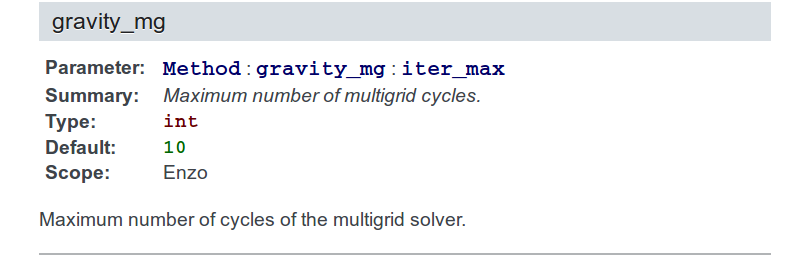
\includegraphics[width=3.5in]{mg_iter_max.png}
\end{center}
\end{frame}

%----------------------------------------------------------------------

\begin{frame}[fragile]
\secframetitle{\ssDevelParameter}
% 
 \bluebf{5.~Access parameter via \greencode{EnzoConfig} class \redcode{enzo\_config}}
\footnotesize
 \begin{semiverbatim}
\bluecode{Method} * \bluecode{EnzoProblem}::\greencode{create_method_} ()
 \{
    if (\redcode{name} == \orangecode{"ppm"}) \{
            \vdots
    \} else if (\redcode{name} == \orangecode{"gravity_mg"}) \{
       \redcode{method} = new \bluecode{EnzoMethodGravityMg0}
 	             (\redcode{field_descr}, \redcode{rank},
                    \vdots
                \redcode{enzo_config}->\redcode{method_gravity_mg_iter_max},
                    \vdots
               );
     \} \ldots
\}

\end{semiverbatim}
\end{frame}
% 
